\chapter{Introduzione}
\label{chapter1}

Lo scopo della cybersecurity è di proteggere i servizi, i dispositivi, le applicazioni e le infrastrutture che usiamo giornalmente. Quindi qualsiasi cosa che usiamo rientra nella cybersecurity. Si differenzia dell'information security in quanto questa mira a proteggere solo le informazioni. La cybersecurity cerca di garantire:
\begin{itemize}
    \item Confidentiality: mira a proteggere la risorsa da accessi non autorizzati. Principalmente si utilizzano, per garantirla, la crittografia e i meccanismi di controllo degli accessi;
    \item Integrity: può essere associata a software, dati, documenti, traffico di rete. Mira a proteggere da modifiche non autorizzate. Si utilizzano principalmente funzioni di hash per verificare possibili manomissioni;
    \item Avaibility: mira a garantire l'accesso delle risorse agli utenti legittimi. SI utilizza principalmente la ridondanza, installando il servizio su più server;
    \item Authenticity: mira a garantire che, nel caso dell'utente, l'utente sia che dice di essere. Si possono usare login con password o tramite dispositivi biometrici. Per i dati viene garantita tramite chiave;
    \item Accountability: si occupa di monitorare chi o cosa compie quali azioni all'interno del sistema. Si utilizzano principalmente i log;
    \item Safety: si assicura che le macchine non causino danno agli operatori che le utilizzano (es: attacco alle centrali elettriche in Ukraina). 

\end{itemize}

\section{Concetti fondamentali}

\paragraph*{Asset} Un asset è qualsiasi cosa che ha valore per un'organizzazione (es: software prodotto, reputazione dell'azienda), un individuo (es: dati personali) o una nazione (es: infrastrutture per la distribuzione elettrica). L'asset può essere materiale o immateriale.

\paragraph*{Vulnerabilità} Una vulnerabilità è una debolezza che gli attaccanti possono usare per danneggiare un asset.

\paragraph*{Cyber threat} Una minaccia è una qualsiasi circostanza/evento che può potenzialmente impattare in modo negativo l'organizzazione.

\paragraph*{Attacco} Un attacco è la realizzazione di una specifica minaccia ad un asset.

\paragraph*{Threat Actor} L'attaccante è colui che esegue l'attacco.

\paragraph*{Rischio} Il rischio quantifica l'impatto che l'attacco avrebbe sull'organizzazione, nonché la probabilità che l'attacco venga effettuato contro l'organizzazione.

\paragraph*{Security controls} Le misure di sicurezza sono un insieme di meccanismi/regole messe in campo per poter proteggere l'asset.

\section{Categorie di attaccanti}

\paragraph{Cybercriminali} sono principalmente spinti da motivazioni economiche. Si concentrano su due tipologie di informazioni: informazioni personali delle vittime (es: info sui clienti dell'azienda) oppure finanziarie (es: carte di credito, credenziali dei conti). 

\noindent Usano generalmente:
\begin{itemize}
    \item Attacchi malware, attuati principalmente con financial trojan, che sono malware che si concentrano sul recuperare le informazioni finanziarie che usano per effettuare transazioni bancarie non autorizzate;
    \item Attacchi ransomware, con cui con cifrano le macchine delle vittime e richiedono un riscatto in cambio della chiave di decifratura;
    \item Attacchi alle vulnerabilità dei sistemi;
    \item Attacchi DDoS con cui rendono non disponibili, ad esempio, dei servizi web e richiedono un riscatto per farli ritornare operativi.
\end{itemize}

\noindent Questi attacchi vengono generalmente attuati usando malware, email di phishing (contengono un link a un sito infetto o un allegato malevolo) o botnet (trasformano il dispositivo in uno zombi in attesa di comandi dell'attacante. Negli attacchi DDoS vengono usati per generare elevato traffico contro il sito bersaglio). Generalmente i malware usati non vengono scritti dai cybercriminals, ma piuttosto comprati. Lo stesso vale per i siti host. 
    
\paragraph{Nation state} gruppi di hacker affiliati ad una potenza governativa mondiale. I loro obiettivi sono principalmente strutture critiche di altri paesi. Le motivazioni sono principalmente due: sabotare infrastrutture o influenzare opinioni politiche/religione nella nazione bersaglio.

\noindent Usano generalmente:
\begin{itemize}
    \item Attacchi malware, per sabotare le strutture critiche;
    \item Campagne di phishing, per ottenere informazioni riservate;
    \item Attacchi DDoS, per non rendere disponibili le strutture critiche.
\end{itemize}

\noindent Questi attacchi vengono attuati tramite malware molto sofisticati e tecniche di evasione per non essere rilevati; utilizzano anche vulnerabilità non ancora note pubblicamente (zero-days vulnerabilities).
    
\paragraph{Attivisti} sono motivati dalla volontà di imporre le proprie visioni religiose, politiche e sociali. Attaccano principalmente quelle organizzazioni non sono in linea con i loro ideali.

\noindent Usano generalmente:
\begin{itemize}
    \item  Web defacement, in cui modificano l'aspetto di un sito web (in cui di solito pubblicano un messaggio);
    \item Rilascio di info confidenziali;
    \item Attacchi DDoS.
\end{itemize}

\noindent Questi attacchi vengono attuati tramite botnet, email infette o vulnerabilità conosciute (exploit kit).
    
\paragraph{Insider Threat} si tratta principalmente di persone che sono state licenziate dall'azienda, o comunque ci hanno avuto dei problemi, che, grazie ai permessi che possiedono, eseguono azioni ai danni dell'azienda stessa. 
    
\noindent Possono:
\begin{itemize}
    \item Rubare e vendere informazioni;
    \item Rilasciare informazioni pubblicamente;
    \item Installare bombe logiche.
\end{itemize}

\noindent Questa categoria comprende anche quei membri dell'azienda che provocano danni involontariamente, pubblicando, ad esempio, per errore file classificati oppure visitando un sito malevolo che andrà ad infettare il network dell'azienda.

\section{Attacchi di tipo Supply chain}

La supply chain si riferisce all'ecosistema di processi, persone, organizzazioni e distributori coinvolti nella creazione e consegna di un prodotto finale. 
Questo tipo di attacchi si sta diffondendo molto in quanto le aziende esternalizzano una parte (o tutto) il ciclo di vita del servizio o dell'applicazione che offre. Ad esempio un software sviluppato modularmente  può fare uso di plug-in sviluppati da terzi, oppure l'infrastruttura su cui il software si appoggia appartiene a terzi (es: cloud).
Gli attaccanti stanno sfruttando le vulnerabilità di questi elementi terzi per attaccare i fruitori del software/servizio fornito dall'azienda.

\noindent Gli elementi chiave della supply chain sono:
\begin{itemize}
    \item Fornitore: fornisce il servizio/software/infrastruttura;
    \item Asset del fornitore: rappresenta elementi di valore che il fornitore usa per produrre il prodotto e che sono bersagli degli attacchi;
    \item Cliente: colui che usufruisce del prodotto del fornitore;
    \item Asset del cliente: elementi di valore posseduti dal cliente che sono l'obiettivo ultimo degli attacchi.
\end{itemize}

\noindent Gli attacchi di \textit{supply chain} si compongono di due parti: una prima parte dove l'attaccante compromette uno o più asset del fornitore sfruttando una vulnerabilità e una seconda parte dove l'attaccante sfrutta gli asset infetti (e la fiducia che il cliente ha nel fornitore) per mettere in campo l'attacco vero e proprio e colpire l'asset del cliente.

Nella figura \ref{fig:my_label} sono riportati gli asset bersaglio del fornitore e i relativi attacchi, mentre nella figura \ref{fig:my_label2} sono riportati gli asset del cliente e i relativi attacchi.

\begin{figure}
    \centering
    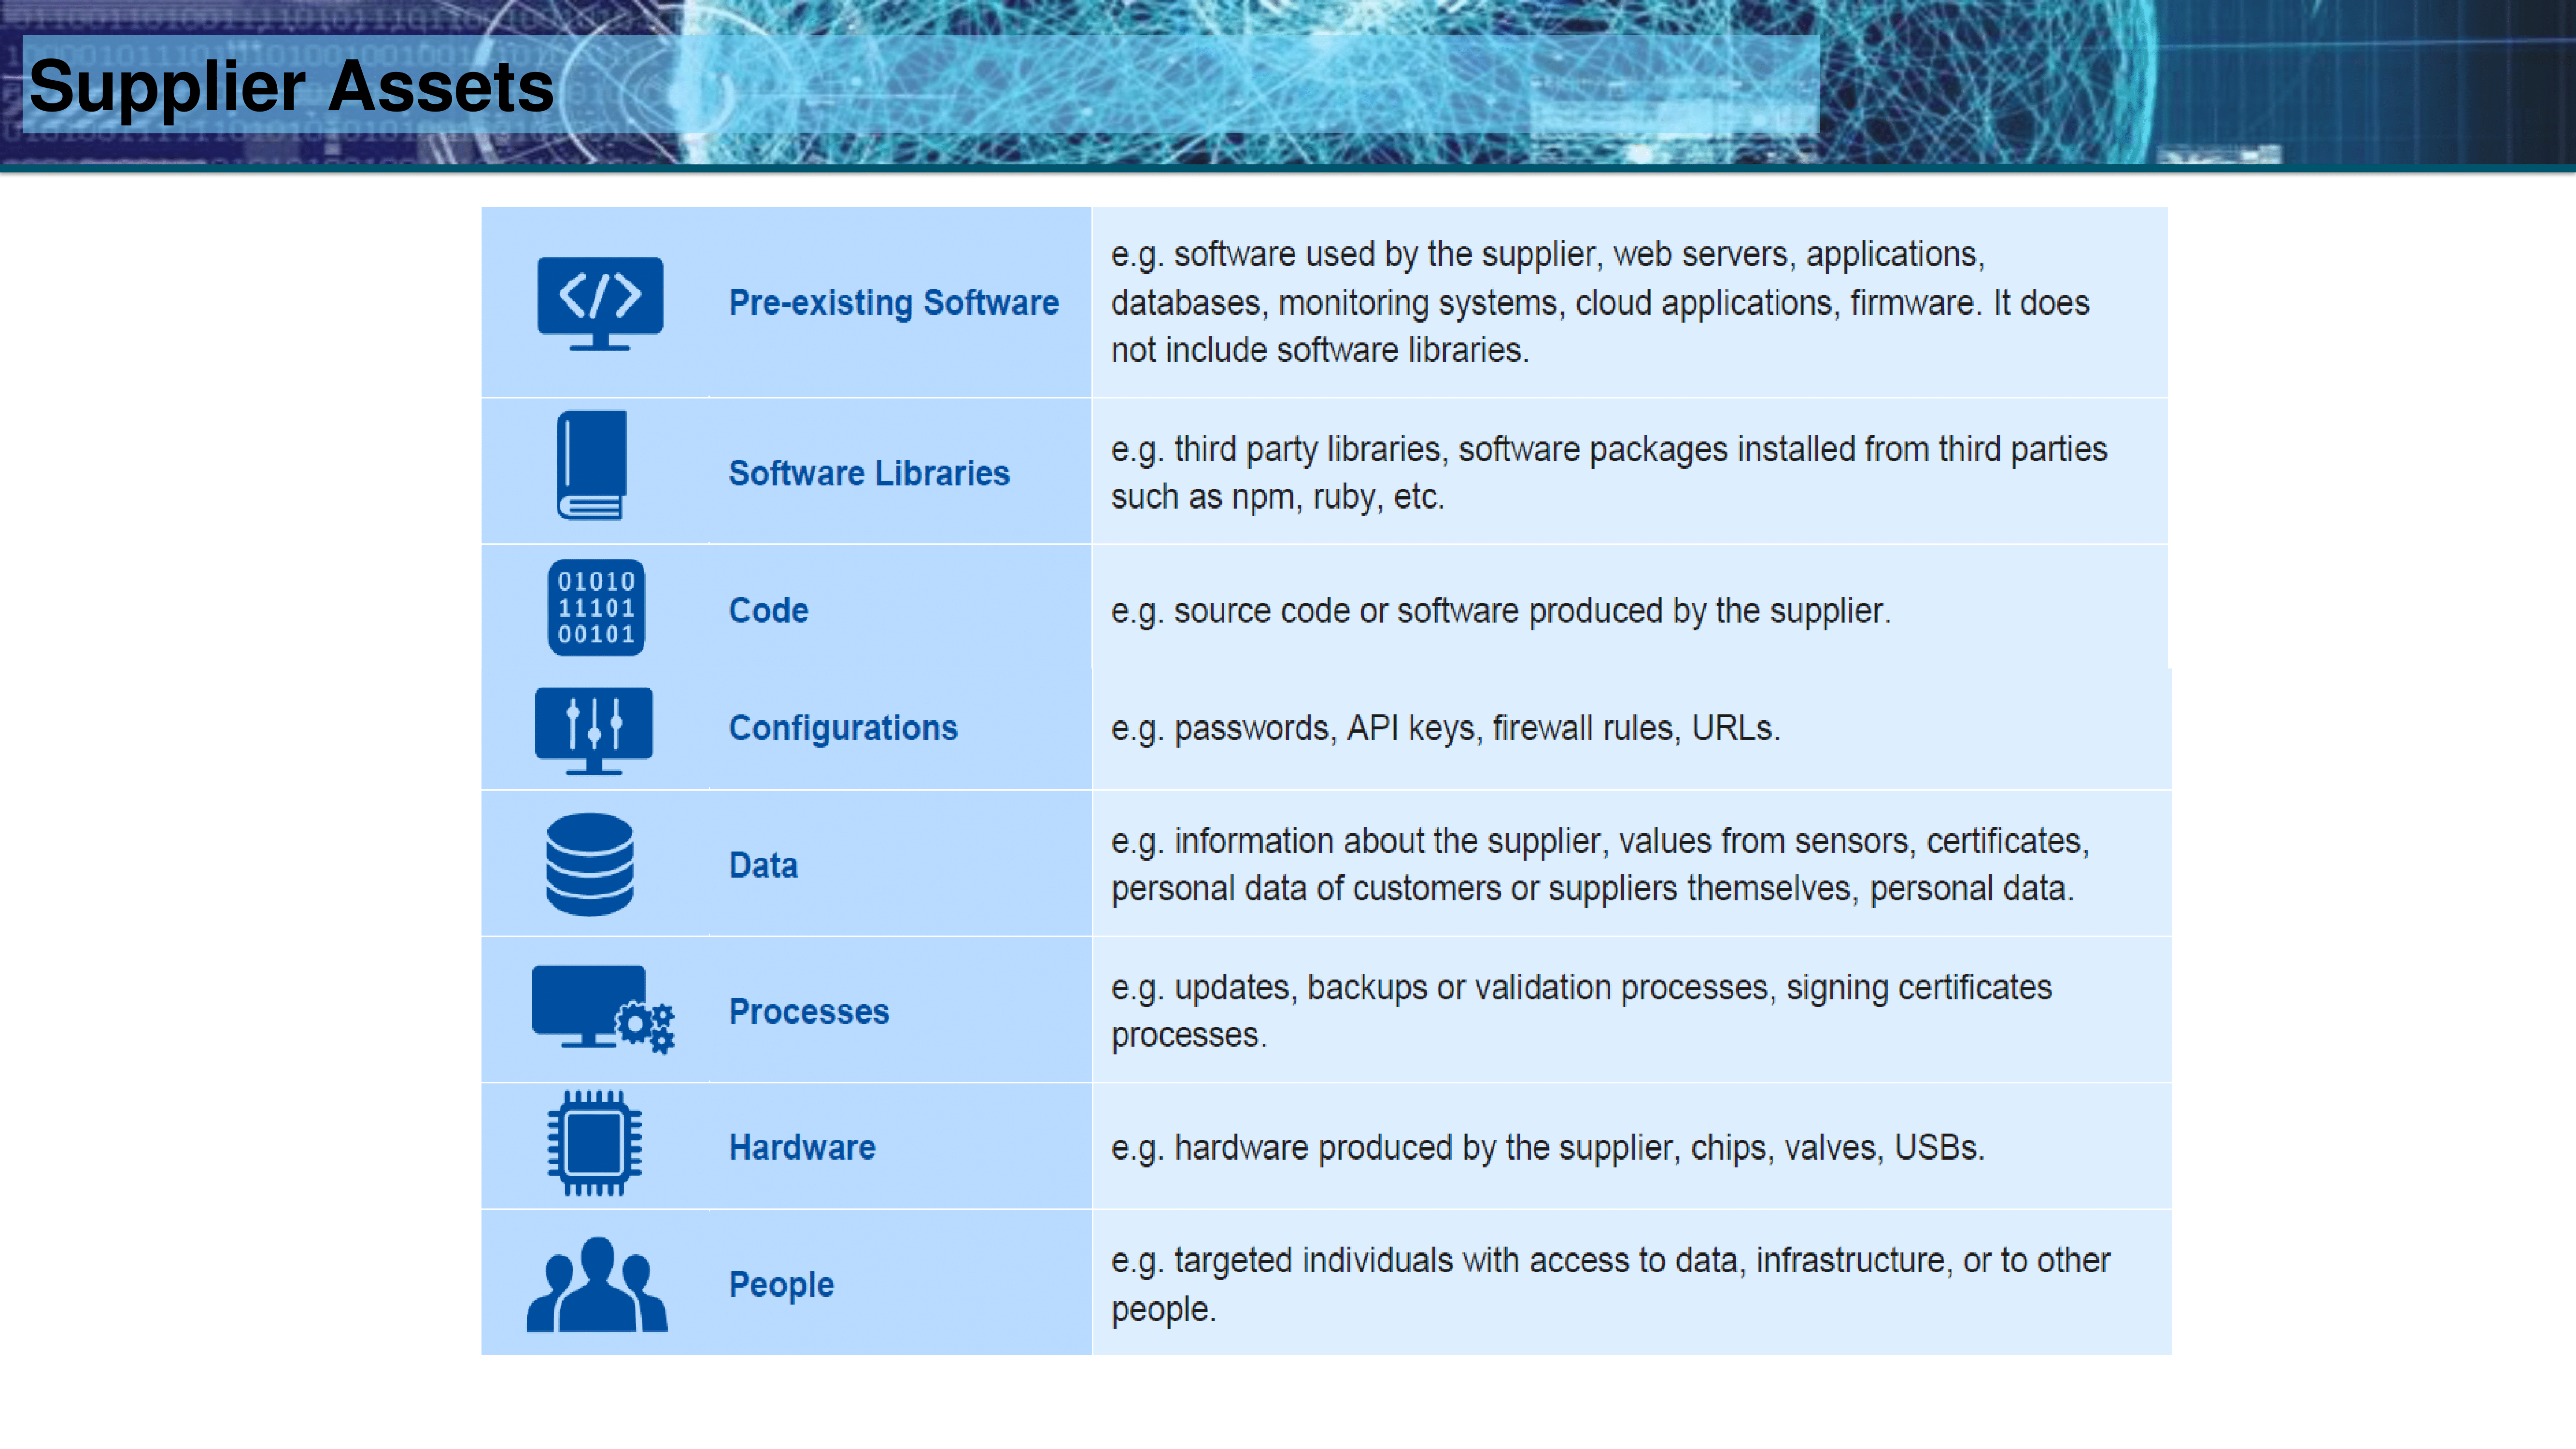
\includegraphics[width=1\textwidth]{images/1.png}
    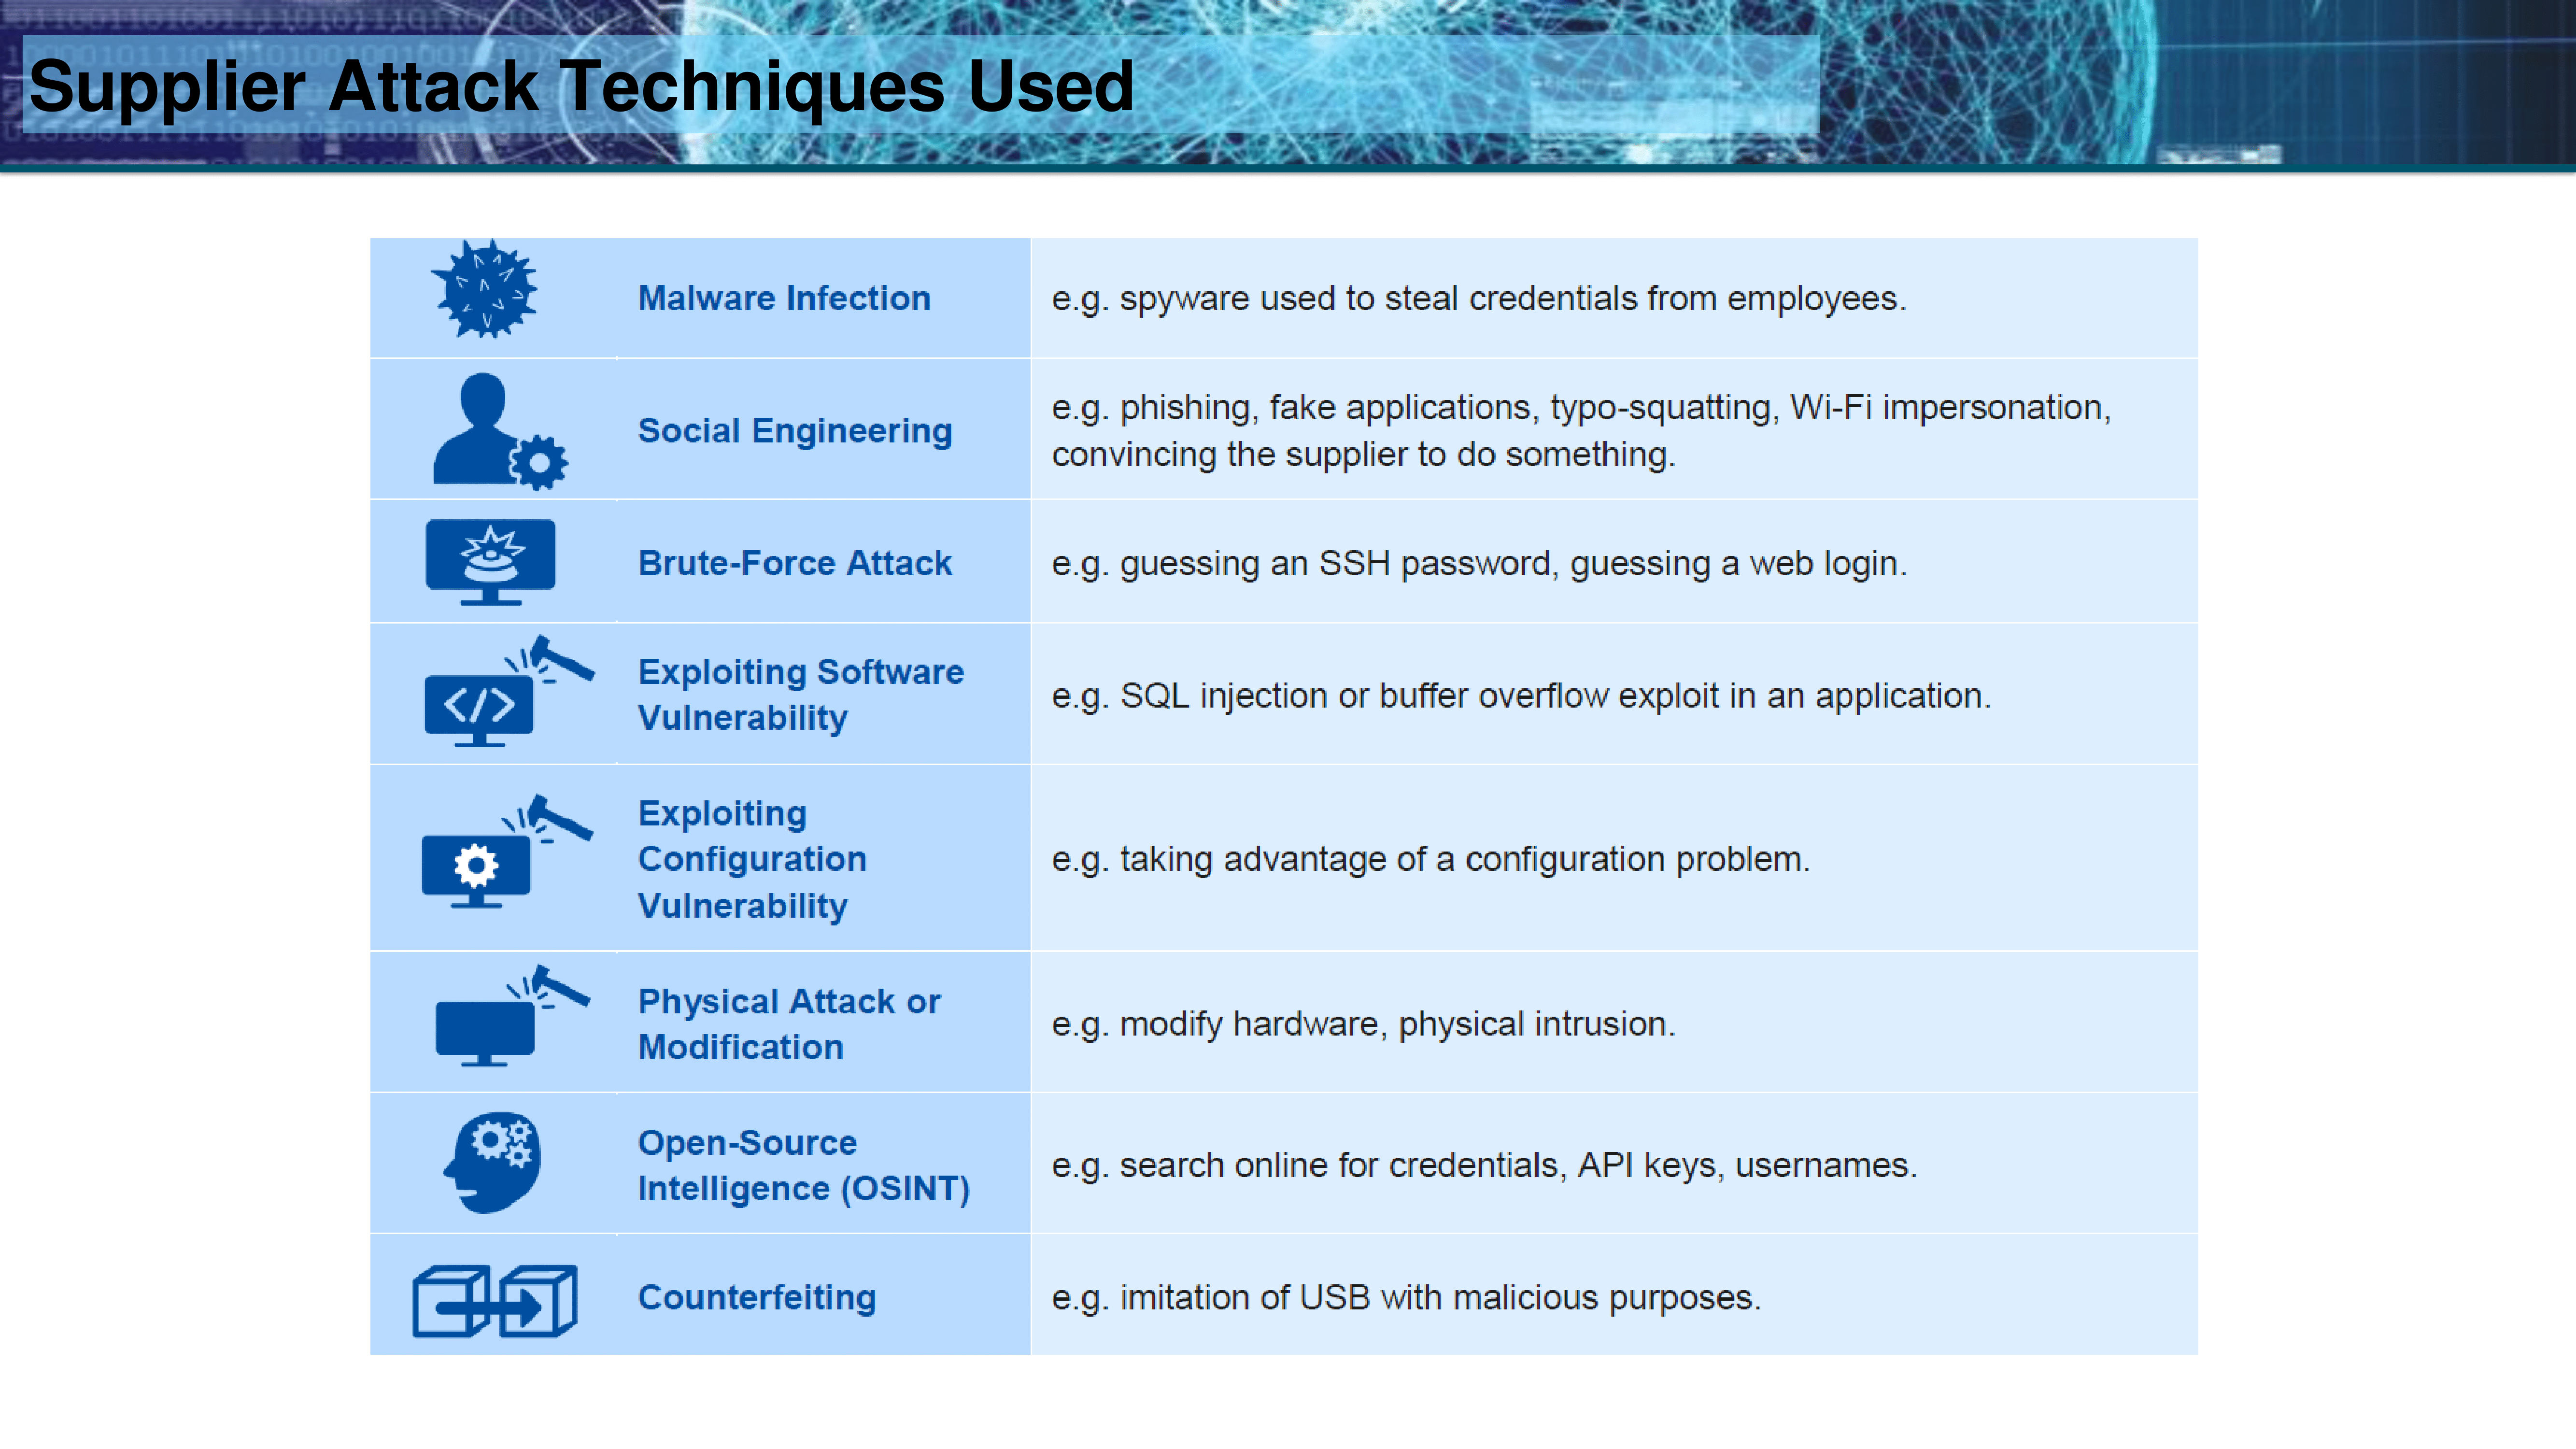
\includegraphics[width=1\textwidth]{images/2.png}
    \caption{Fornitore}
    \label{fig:my_label}
\end{figure}

\begin{figure}
    \centering
    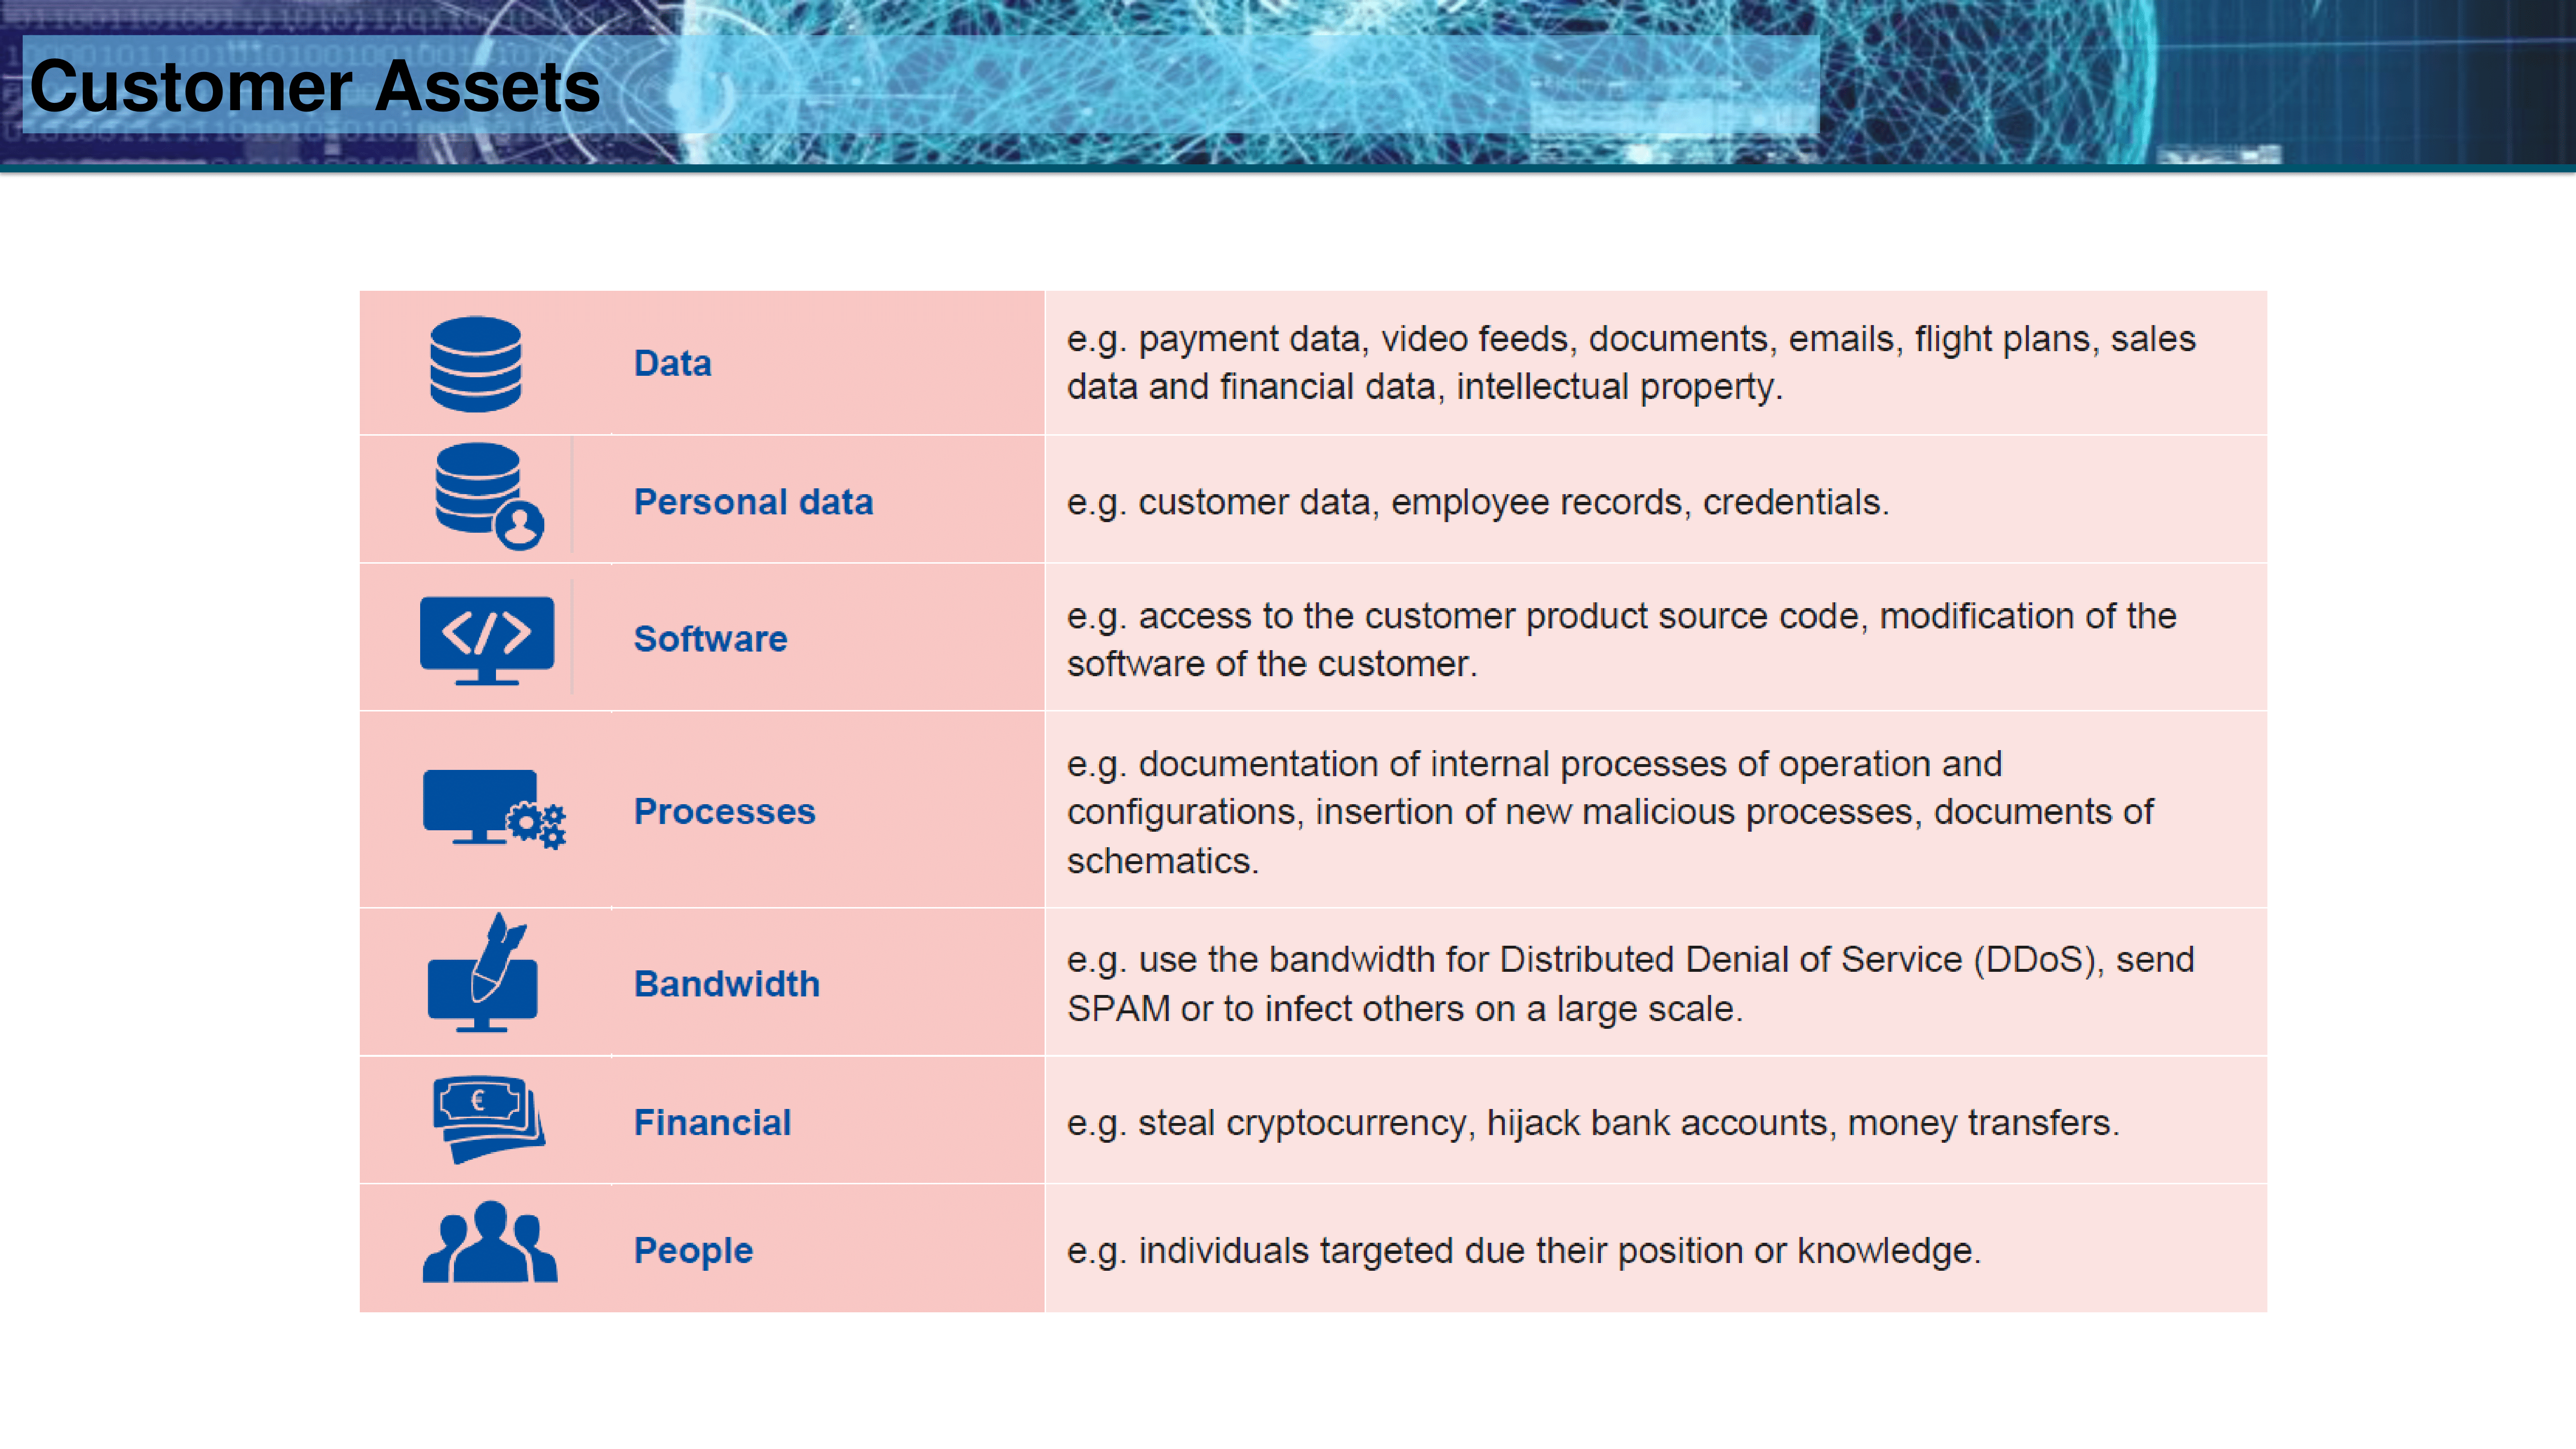
\includegraphics[width=1\textwidth]{images/3.png}
    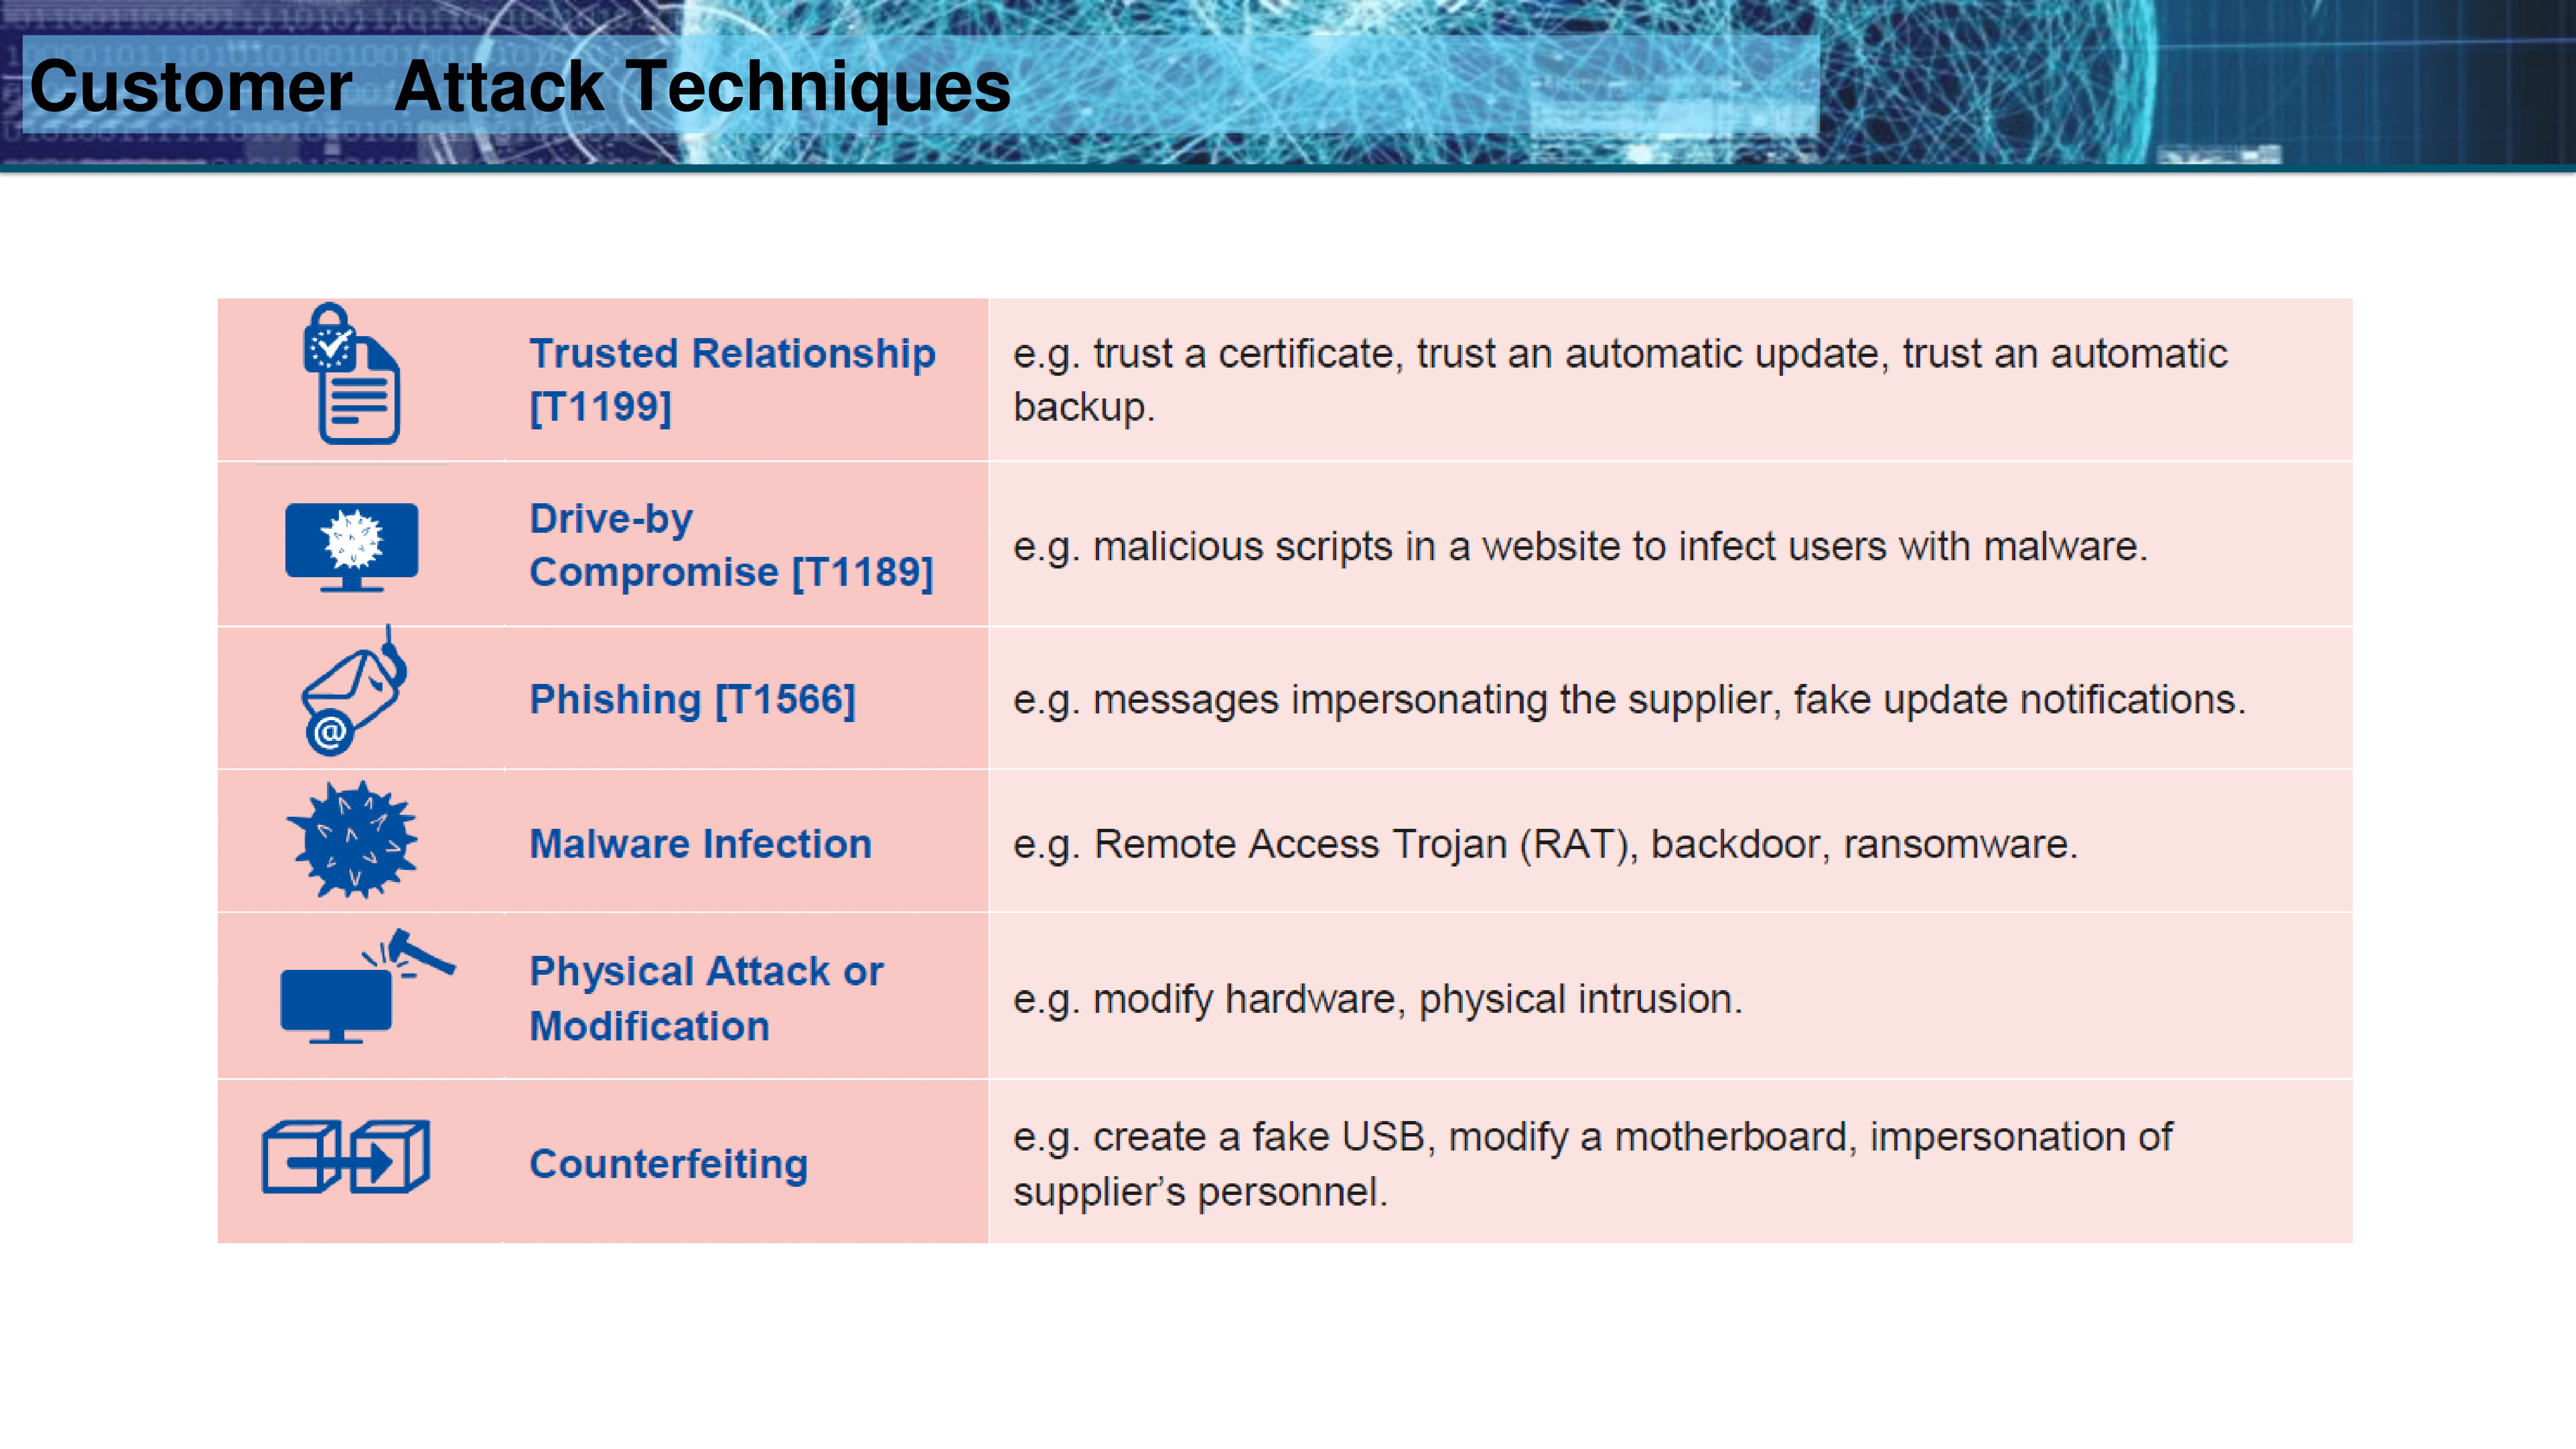
\includegraphics[width=1\textwidth]{images/4.png}
    \caption{Cliente}
    \label{fig:my_label2}
\end{figure}

\section{SolarWinds}
L'attacco è stato scoperto nel 2021 da un'azienda da cybersecurity. Il tutto è partito con la compromissione di un software di nome Orion, prodotto da SolarWind. Viene usato per il management di rete. Ha la caratteristica di comunicare con qualsiasi dispositivo sulla rete, inviare loro comandi e raccogliere informazioni. L'attacco di attribuisce ad APT29, un gruppo di nation state associato al governo russo.

L'attacco ha compromesso il processo di aggiornamento del software, andando ad installare su tutte le macchine che lo usavano un aggiornamento malevolo. L'aggiornamento andava poi a installare un malware sulle macchine che andava a raccogliere dati sensitivi delle vittime. 
\\

\noindent L'attacco è stato portato avanti in più fasi:
\begin{enumerate}
    \item Infiltrazione iniziale: gli attaccanti hanno raccolto info su SolarWinds e in particolare hanno hanno fatto reconnaissance sfruttando una vulnerabilità del Microsoft Exchenge Server (che gestisce le comunicazione di posta elettronica). Grazie a questa sono riusciti ad accedere alla mail dei dipendenti e recuperare le credenziali di accesso. Da questo sono riusciti a monitorare le comunicazioni e capire come funzionava il sistema di aggiornamento di Orion;
    \item Spear phishing: gli attaccanti hanno attuato una campagna di spear phishing contro i dipendenti che avevano accesso ai server usati per effettuare gli aggiornamenti e le loro distribuzione. Le mail contenevano una allegato malevolo che andava a installare un malware sulle macchine. Questo malware andava a monitorare i processi in esecuzione sulle macchine dedicati alla compilazione degli aggiornamenti e al caricamento delle build sul server degli aggiornamenti. Una volta identificato il processo di aggiornamento, il malware è andato a copiare un secondo malware (la vera arma) in più file coinvolti nel processo di aggiornamento;
    \item Weaponization: quando i clienti aggiornavano Orion, andavano a scaricare l'aggiornamento malevolo che conteneva una backdoor che dava accesso di amministratore agli attaccanti. Il malware, una volta scaricato, restava dormiente per 2 settimane prima di tentare di comunicare con Command and Control server in attesa di comandi dagli attaccanti. 
\end{enumerate}









